\documentclass[aspectratio=169]{beamer}

% SETUP =====================================
\usepackage[T1,T2A]{fontenc}
\usepackage[utf8]{inputenc}
\usepackage[russian]{babel}
\usepackage{listings}
\usepackage{array}
\usepackage{amssymb}
\usepackage{pifont}
\usepackage{minted}
\usepackage{pgf-pie}
\usepackage{fancyvrb}
\usepackage{../../beamerthemeslidesgeneric}
% SETUP =====================================

\title{Scala Ecosystem}
\author{Mikhail Mutcianko, Alexey Otts}
\institute{СПБгУ, СП}
\date{\today}

\begin{document}

\frame{\titlepage}

\section{Overview \\ \footnotesize as of Apr 2020}

\begin{frame}{Scala versions}
  {Which versions of Scala do you regularly use?}
  \begin{figure}[htpb]
    \begin{center}
      \begin{tikzpicture}[scale=0.8, transform shape]
      \pie[sum=auto,after number=\%]{1/Dotty, 13/2.10, 20/2.13, 36/2.11, 68/2.12}
      \end{tikzpicture}
    \end{center}
  \end{figure}
\end{frame}

\begin{frame}{JVM Platform}
  {Which versions of Java do you regularly use?}
\begin{figure}[htpb]
  \begin{center}
    \begin{tikzpicture}[scale=0.8, transform shape]
    \pie[sum=auto,after number=\%]{73/Java 8, 28/Java 11, 13/Java 10, 11/Java 9}
    \end{tikzpicture}
  \end{center}
\end{figure}  
\end{frame}

\begin{frame}{Testing}{Which unit-testing frameworks do you regularly use?}
\begin{figure}[htpb]
  \begin{center}
    \begin{tikzpicture}[scale=0.8, transform shape]
    \pie[sum=auto,after number=\%]{5/None, 3/TestNG, 8/specs2, 10/µTest, 14/ScalaMock,
    15/ScalaCheck, 26/JUnit, 77/ScalaTest}
    \end{tikzpicture}
  \end{center}
\end{figure}
\end{frame}

\begin{frame}{Most Popular Libraries}
  {Which frameworks / libraries do you regularly use?}
\begin{figure}[htpb]
  \begin{center}
    \begin{tikzpicture}[scale=0.8, transform shape]
    \pie[sum=auto,after number=\%]{55/Akka, 40/Spark, 17/Slick, 13/Shapeless, 13/Cats, 12/Scalaz}
    \end{tikzpicture}
  \end{center}
\end{figure}
\end{frame}

\begin{frame}{Build System}{Which build systems do you regularly use?}
\begin{figure}[htpb]
  \begin{center}
    \begin{tikzpicture}[scale=0.8, transform shape]
      \pie[sum=auto,after number=\%]{71/sbt, 39/Maven, 18/Gradle, 3/Pants, 2/Ant, 2/Bazel}
    \end{tikzpicture}
  \end{center}
\end{figure}
\end{frame}

\section{SBT}

\begin{frame}{What is a build system?}
  Build system is a tool to help automate development processess such as compilation of source
  coude, running tests and deploying the resulting application.
\end{frame}

\begin{frame}{Real world projects}
  \begin{itemize}
    \item $n*10^5 - n*10^6 LOC$
    \item 10-1000 developers on the same codebase
    \item $n*10^5$ tests
    \item 10-100 steps to build the final application
  \end{itemize}
\end{frame}

\begin{frame}{The problem}
  Given: n source files \\
  Basic tasks:
  \begin{itemize}
    \item compile sources to class files
    \item find classes that are tests and run? them
    \item run the application from classes
  \end{itemize}
\end{frame}

\begin{frame}{Build tool interface}
\begin{itemize}
  \item command line: \texttt{sbt ;compile;test;}, \texttt{mvn install}, \texttt{make -j8}
  \item configuration: Makefile, build.sbt, pom.xml
  \item remote API: gradle-daemon, sbt-server, BSP
\end{itemize}
\end{frame}

\begin{frame}{sbt}{simple build tool}
  \begin{itemize}
    \item build files are defined in Scala
    \item incremental compilation
    \item test framork integrations
    \item build jar artifacts and publish them
    \item \ldots
  \end{itemize}
\end{frame}

\begin{frame}[fragile]{Project structure}
\begin{verbatim}
build.sbt
src/
  main/
    resources/ <files to include in main jar here>
    scala/     <main Scala sources>
    java/      <main Java sources>
  test/
    scala/     <test Scala sources>
    java/      <test Java sources>
target/        <build results>
\end{verbatim}
\end{frame}

\begin{frame}{SBT command line basics}
  \begin{itemize}
    \item run sbt in your project directory with no arguments:\\ \texttt{\$ sbt}
    \item specify tasks to run:\\ \texttt{\$ sbt clean compile "testOnly TestA TestB"}
    \item common commands:
      \begin{itemize}
        \item reload --- Reloads the build definition
        \item clean --- Deletes all generated files (in the target directory)
        \item compile --- Compiles the main sources
        \item test --- Compiles and runs all tests
        \item console --- run interpreter with a classpath including the compiled sources
          and all dependencies
      \end{itemize}
  \end{itemize}
\end{frame}

\begin{frame}[fragile]{Build defiinition}
The build definition is described in \texttt{build.sbt} (actually any files named *.sbt) in the project’s
base directory. SBT build definitions consists of:

\begin{itemize}
  \item a set of subproject definitions \\
    \begin{minted}{scala}
lazy val root = (project in file(".")).settings(
    name := "Hello",
    scalaVersion := "2.12.7") 
    \end{minted}
  \item setting expressions \\
\begin{minted}{scala}
ThisBuild / organization := "com.example"
ThisBuild / scalaVersion := "2.12.10"
ThisBuild / version      := "0.1.0-SNAPSHOT"
\end{minted}
\end{itemize}
\end{frame}

\begin{frame}[fragile]{SBT Settings}
Settings are a sequence of key-value pairs generated by setting operators.
\begin{center}
  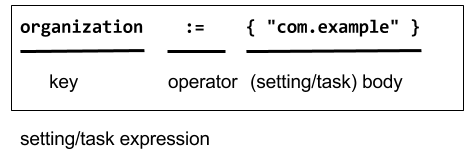
\includegraphics[scale=0.3]{setting-expression}
\end{center}
\begin{itemize}
  \item 3 kinds of keys:
    \begin{itemize}
      \item \texttt{SettingKey[T]} --- a key for a value computed once
      \item \texttt{TaskKey[T]} --- a key for a value, called a task, that has to be recomputed each
        time, potentially with side effects
      \item \texttt{InputKey[T]} --- a key for a task that has command line arguments as input
    \end{itemize}
\end{itemize}
\end{frame}

\begin{frame}{Key initialization operators}
\begin{itemize}
  \item \texttt{:=} --- initialize key discarding prevoius value
  \item \texttt{+=} --- append single element to prevoius value
  \item \texttt{++=} --- append a collection to prevoius value
\end{itemize}
\end{frame}

\begin{frame}[fragile]{SBT Task Graph}
Rather than thinking of settings as key-value pairs, a better analogy would be to think of it as a
directed acyclic graph (DAG) of tasks where the edges denote happens-before. Let’s call this the
task graph.

\begin{itemize}
  \item depend on other values by using \texttt{.value method}
  \item setting keys cannot depend on tasks
  \item show key dependencies with \texttt{inspect} task
\end{itemize}
\end{frame}

\begin{frame}[fragile]{SBT Task Graph}
\begin{minted}{scala}
scalacOptions := {
  val ur = update.value  // update task happens-before scalacOptions
  val x = clean.value    // clean task happens-before scalacOptions
  // ---- scalacOptions begins here ----
  ur.allConfigurations.take(3)
}
\end{minted}
\end{frame}

\begin{frame}[fragile]{Scopes}
Previously we pretended that a key like name corresponded to one entry in sbt’s map of key-value
pairs. This was a simplification.
In truth, each key can have an associated value in more than one context, called a scope
\begin{itemize}
  \item a key can have a different value in each project
  \item compile key has a different value for main and test sources
  \item a global key can be "overridden" in a project
\end{itemize}
\vspace{1em}
\begin{center}
  \begin{minted}{scala}
  projA / Compile / console / scalacOptions
  \end{minted}
\end{center}
\end{frame}

\begin{frame}{Scope Axis}
  \begin{itemize}
    \item subproject axis
    \item configuration axis
    \item task axis
  \end{itemize}
\end{frame}

\begin{frame}[fragile]{Subprojects}
  A project is defined by declaring a lazy val of type Project. For example, :
  \vspace{2em}
  \begin{minted}{scala}
lazy val core = (project in file("core"))
  .settings(
    // other settings
  )

lazy val util = (project in file("util"))
  .settings(
    // other settings
  ).dependsOn(core)
  \end{minted}
\end{frame}

\begin{frame}[fragile]{Aggregation and Dependencies}
\begin{block}{Aggregation}
Aggregation means that running a task on the aggregate project will also run it on the aggregated
projects
\end{block}
\begin{minted}{scala}
lazy val root = (project in file(".")).aggregate(util, core)

lazy val util = (project in file("util"))
lazy val core = (project in file("core"))
\end{minted}
\pause
\begin{block}{Classpath dependencies}
A project may depend on code in another project. This is done by adding a dependsOn method call
\end{block}
\end{frame}

\begin{frame}[fragile]{Classpath dependencies}
\begin{minted}{scala}
lazy val util = (project in file("util"))

lazy val core = (project in file("core"))
  .dependsOn(util)

lazy val app = (project in file("app"))
  .dependsOn(core % "test->test;compile->compile")
\end{minted}
\end{frame}

\begin{frame}{Configurations}
\begin{itemize}
  \item \texttt{Compile} which defines the main build (src/main/scala).
  \item \texttt{Test} which defines how to build tests (src/test/scala).
  \item \texttt{Runtime} which defines the classpath for the run task. 
\end{itemize}
\end{frame}

\begin{frame}[fragile]{Referring to scopes}
  Key scoping is done using the "/" operator:
\begin{minted}{scala}
organization := name.value
Compile / name := "hello"
packageBin / name := "hello"
Compile / packageBin / name := "hello"
\end{minted}
\end{frame}

\begin{frame}[fragile]{Library dependencies}
\begin{block}{Unmanaged dependencies}
Jar files that are assumed to already exist in the filesystem
\end{block}
\begin{minted}{scala}
unmanagedBase := baseDirectory.value / "custom_lib_folder"
unmanagedJars += baseDirectory.value / "myLib.jar"
\end{minted}
\pause
\vspace{1em}
\begin{block}{Managed dependencies}
Dependencies that are managed by some dependendency management programs such as Coursier or Apache
Ivy
\end{block}
\begin{minted}{scala}
// libraryDependencies += groupID % artifactID % revision % configuration
libraryDependencies += "org.apache.derby" % "derby" % "10.4.1.3"
\end{minted}
\end{frame}

\begin{frame}[fragile]{Managed dependencies}
  \begin{itemize}
    \item \texttt{libraryDependencies} is a pre-defined key in \texttt{sbt.Keys}:\\
    \hskip-1em \mintinline{scala}{libraryDependencies = settingKey[Seq[ModuleID]]("Declares managed dependencies.")}
    \item \texttt{\%} is an extension method of \texttt{String} thar creates a \texttt{ModuleID}
    \item \texttt{\%\%} inserts binary Scala version suffix into the artifact id:\\
      \begin{minted}{scala}
      libraryDependencies += "org.scala-tools" % "scala-stm_2.11" % "0.3"
      libraryDependencies += "org.scala-tools" %% "scala-stm" % "0.3"
      \end{minted}
    \item use 3rd \texttt{\%} operator to provide scope:
      \begin{minted}{scala}
      libraryDependencies += "org.apache.derby" % "derby" % "10.4.1.3" % "test"
      libraryDependencies += "org.apache.derby" % "derby" % "10.4.1.3" % Test
      \end{minted}
  \end{itemize}
\end{frame}

\begin{frame}[fragile]{Extended build structure}
\vskip-1em
\begin{block}{sbt is recursive}
The \texttt{project} directory is another build inside your build, which knows how to build your build
\end{block}
\begin{Verbatim}[fontsize=\tiny]
  hello/                     # your build's root project's base directory
      Hello.scala         # a source file in your build's root project
      build.sbt              # build.sbt is part of the source code for
                             #   meta-build's root project inside project/;
                             #   the build definition for your build
      project/            # base directory of meta-build's root project
          build.sbt          # this is part of the source code for
                             #   meta-meta-build's root project in project/project;
                             #   build definition's build definition
          project/        # base directory of meta-meta-build's root project;
                          #   the build definition project for the build definition
              MetaDeps.scala # source file in the root project of
                             #   meta-meta-build in project/project/
\end{Verbatim}
\end{frame}

\begin{frame}[fragile]{Tracking dependencies in one place}
  One way of using the fact that .scala files under project is a part of the build is
  to create \texttt{project/Dependencies.scala} to track dependencies in one place.
  \begin{minted}{scala}
object Dependencies {
  lazy val akkaVersion = "2.3.8"
  // Libraries
  val akkaActor = "com.typesafe.akka" %% "akka-actor" % akkaVersion
  val specs2core = "org.specs2" %% "specs2-core" % "2.4.17"
  // Projects
  val backendDeps =
    Seq(akkaActor, specs2core % Test)
} 
  \end{minted}
\end{frame}

\begin{frame}[fragile]{Tracking dependencies in one place}{build.sbt}
\begin{minted}{scala}
import Dependencies._

ThisBuild / organization := "com.example"
ThisBuild / version      := "0.1.0-SNAPSHOT"
ThisBuild / scalaVersion := "2.12.10"

lazy val backend = (project in file("backend"))
  .settings(
    name := "backend",
    libraryDependencies ++= backendDeps
  )
\end{minted}
\end{frame}

\begin{frame}[fragile]{SBT plugins}
  Prts of a build definition can be loaded from classes and jars --- thus creating plugins
  \begin{itemize}
    \item plugins are added with \texttt{addSbtPlugin(...)}:\\
      \mintinline{scala}{addSbtPlugin("com.eed3si9n" % "sbt-assembly" % "0.11.2")}
    \item since plugin runs inside the build itself, it has to be added by the meta-build\\
      e.g. into \texttt{project/plugins.sbt}
    \item some plugins are not enabled automatically:\\
      \begin{minted}{scala}
lazy val util = (project in file("util"))
  .enablePlugins(FooPlugin, BarPlugin)
  .settings(
    name := "hello-util"
  )
      \end{minted}
  \end{itemize}
\end{frame}

\end{document}

